\documentclass[11pt,a4paper]{report}
\usepackage[latin1]{inputenc}
\usepackage{amsmath}
\usepackage{amsfonts}
\usepackage{amssymb}
\usepackage{cite}
\usepackage{graphics, graphicx}
\graphicspath{{Immagini/}}
\usepackage{float}
\usepackage{booktabs}
\author{Chiara Camerota}
\title{Analisi del network dei criminali londinesi}
\begin{document}
	\maketitle
\chapter*{Introduzione}
Il network preso in esame riassume le relazioni tra i membri delle gang londinesi, basandosi sugli atti criminali commessi in gruppo, durante il periodo 2005-2009. I dati vengono forniti in forma anonima dalla polizia, sulla base degli arresti e delle condanne subite dai membri. 
 \\
La rete presenta 54 nodi, ognuno corrispondente ad un membro delle gang, mentre gli archi possono assumere diversi valori, corrispondenti a diversi livelli di criminalit\'a. Nello specifico: 1 indica che i nodi si frequentano, 2 indica che i due hanno commesso atti criminali assieme, 3 che hanno commesso gravi atti criminali assieme, 4 indica la condizione precedente e che vi \'e un legame di parentela tra i due nodi.
\\
Il nostro obbiettivo \'e quello riuscire a capire che ruolo gioca la nazionalit\'a nel commettere atti criminali di gruppo, indi per cui rendiamo binario il nostro network, ovvero diamo pari peso a tutti gli archi.
\\
\begin{figure}[H]
	\centering
		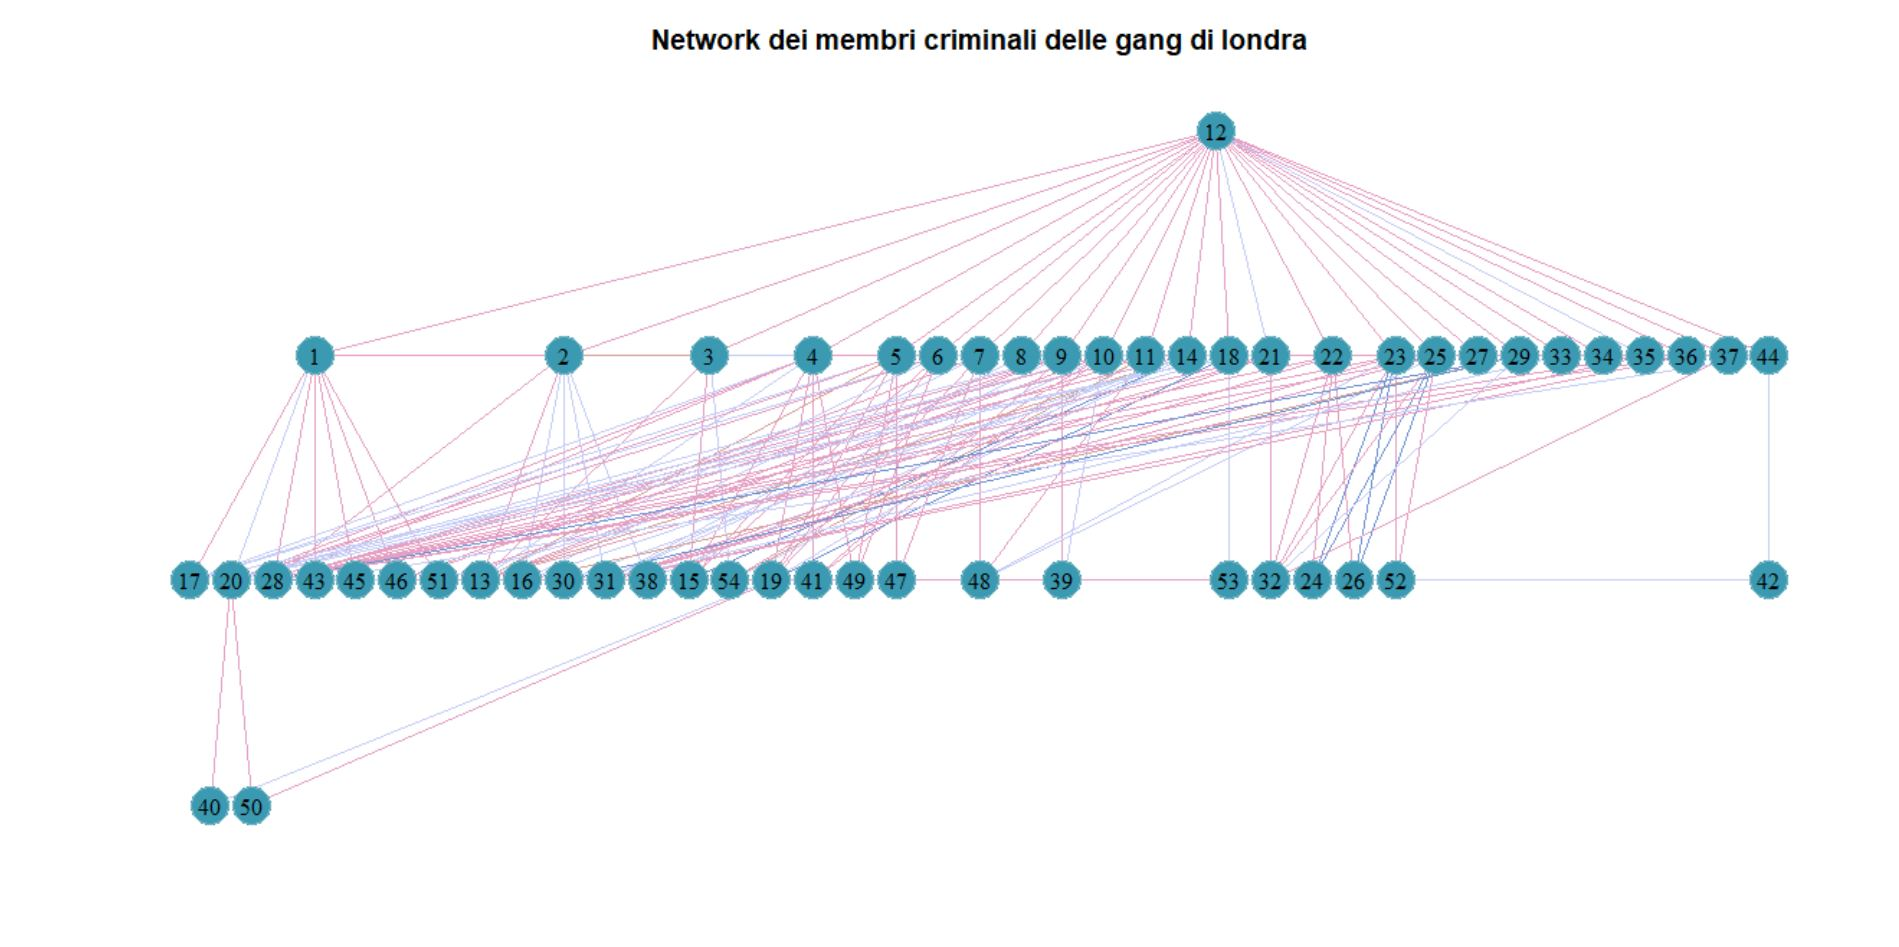
\includegraphics[scale =0.5]{networkviola}
	\caption{Sopra \'e riportato il grafo originale, ogni colore indica un legame diverso tra le unit\'a. Il rosa indica un arco di tipo 1, il blu cobalto chiaro un legame di tipo 2, il marrone uno di tipo 3, il blu cobalto scuro un legame di tipo 4 .Come si pu\'o osservare, il grafo presenta una struttura piramidale, tipica delle organizzazioni criminali.}
	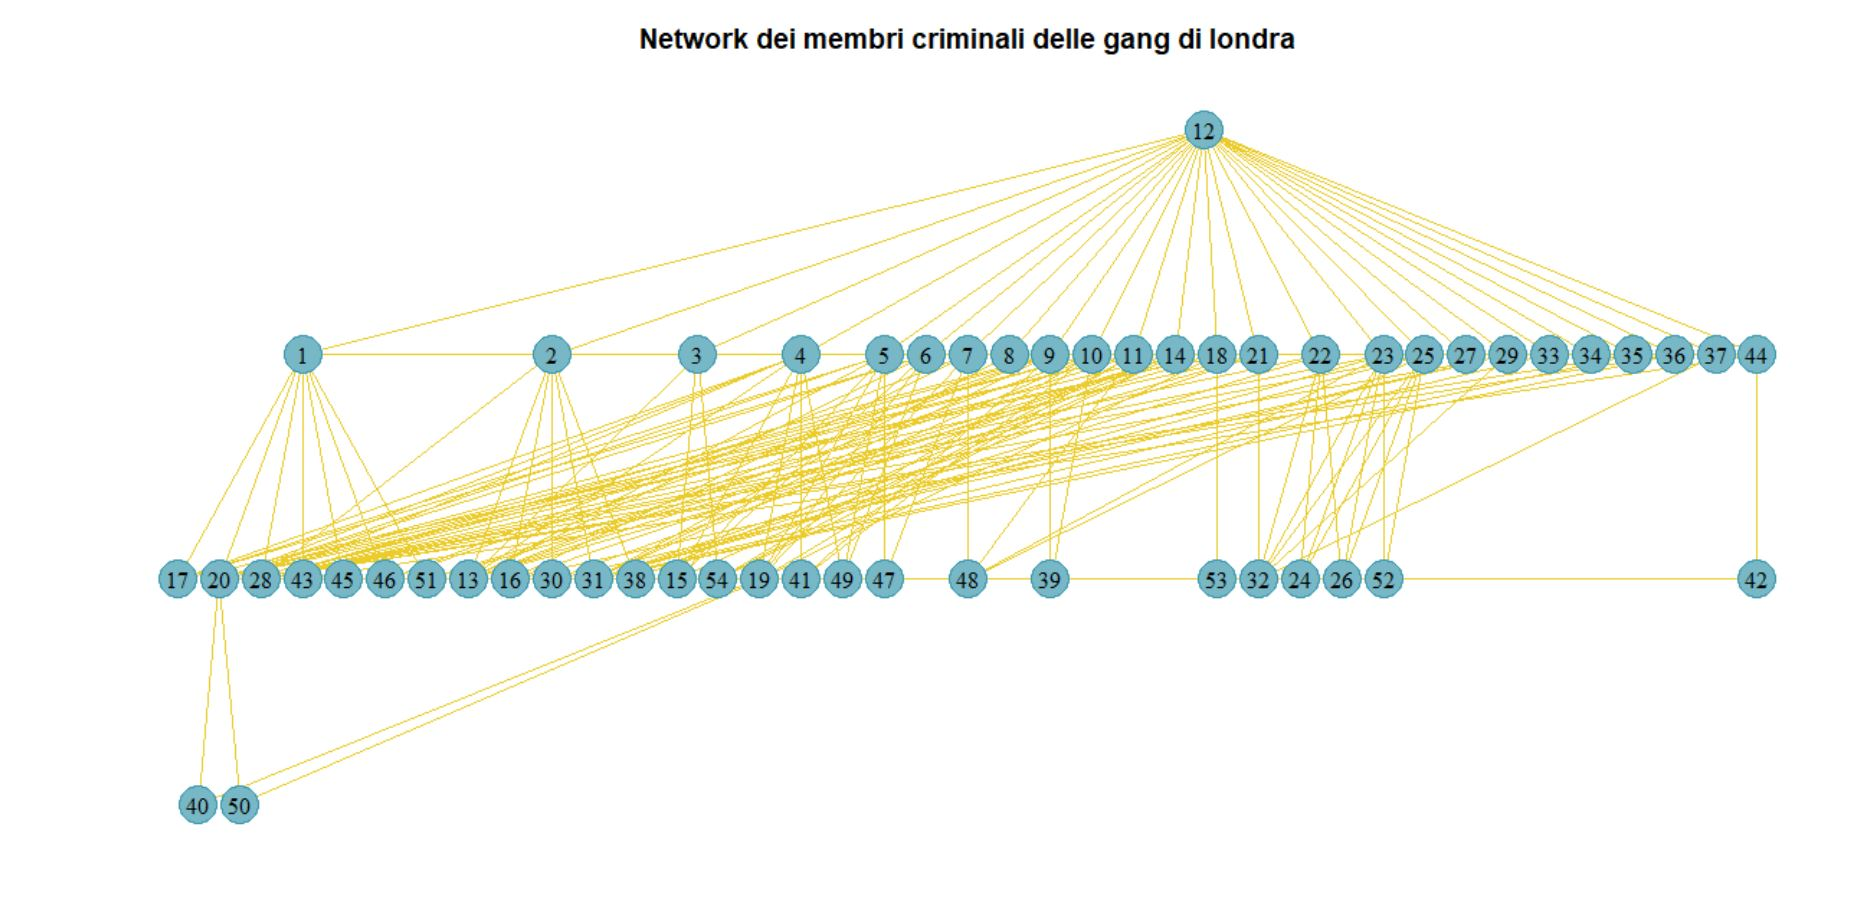
\includegraphics[scale =0.5]{networkbinary}
	\caption{Sopra \'e riportato il grafo dicotomizzato.}

\end{figure}

Gli attributi presi in considerazione sono: l'et\'a, il luogo di nascita, la residenza, il numero degli arresti, il numero di condanne, se il membro \'e o meno in carcere.
\\
Di seguito sono riassunti in tabella le descrittive delle covariate.
\begin{itemize}
	\item \emph{Residence}: vale 1 se il criminale ha la residenza, 0 altrimenti\\\\
\begin{tabular}{c|c|c}
	\hline 
	\textbf{Residence} & 1  & 0  \\ 
	\hline 
	Frequenza & 20  &34  \\ 
	\hline 
\end{tabular} 
	\item \emph{Prison}:  vale 1 se il criminale \'e in prigione, 0 altrimenti\\\\
\begin{tabular}{c|c|c}
	\hline 
	\textbf{Prison} & 1  & 0  \\ 
	\hline 
	Frequenza & 20  &34  \\ 
	\hline 
\end{tabular} 
\\
	\item \emph{BirthPlace}: vale 1 per i nati in Africa dell'ovest , 2 per quelli dei Caraibi, 3 per i nati negli UK, 4 per quelli dell'Africa dell'est \\\\
\begin{tabular}{c|c|c|c|c}
	\hline 
	\textbf{BirthPlace} & 1  & 2 & 3& 4  \\
	\hline 
	Frequenza & 12 & 12 & 24 & 6   \\ 
	\hline 
\end{tabular} 
\\
\item \emph{Age}: indica l'et\'a del criminale \\\\
\begin{tabular}{c|c|c|c|c|c |c}
\hline 
\textbf{Age} & Min. & 1st Qu. & Median &   Mean& 3rd Qu. &   Max.    \\ 
\hline 
Valore &  16.00  & 18.00 &  19.00  & 19.83 &  21.00 &  27.00  \\ 
\hline 
\end{tabular} 
\\
\item \emph{Arrests}: indica il numero di arresti subiti dal criminale \\\\
\begin{tabular}{c|c|c|c|c|c |c}
\hline 
\textbf{Arrests} & Min. & 1st Qu. & Median &   Mean& 3rd Qu. &   Max.    \\ 
\hline 
Valore &  0.000 &  5.000 &  8.000 &  9.907&  14.750&  23.000   \\ 
\hline 
\end{tabular} 
\\
\item \emph{Convictions}: indica il numero di condanne a carico del criminale \\\\
\begin{tabular}{c|c|c|c|c|c |c}
\hline 
\textbf{Convictions} & Min. & 1st Qu. & Median &   Mean& 3rd Qu. &   Max.    \\ 
\hline 
Valore &   0.000 &  1.000 &  3.000 &  4.204 &  7.000 & 13.000   \\ 
\hline 
\end{tabular} 



\end{itemize}
Studi precedenti, come ad esempio Grund, T. and Densley, J. (2012, 2015) dimostrano come sia pi\'u probabile, per due criminali che agiscono insieme, che questi abbino la stessa nazionalit\'a piuttosto che altro in comune; ma vedremo come l'omofilia, ovvero la scelta di commettere atti criminali con persone aventi o meno la propria nazionalit\'a, \'e molto pi'u forte nelle triadi, piuttosto che nelle 2-star. Una possibile spiegazione di questo fenomeno \'e che per due criminali (aventi la stessa nazionalit\'a) \'e pi\'u semplice trovare un amico in comune all'interno di questo gruppo, piuttosto che all'esterno.
\chapter{Analisi descrittive e Studio della centralit\'a}
\subsection{Densit\'a, Censimento delle triadi, transitivit\'a ed assortative mixing}
Iniziamo ora l'analisi descrittiva della rete, come prima cosa possiamo notare che la rete non direzionata ha 54 nodi collegati tra di loro mediante 315 archi, sui $\binom{54}{2}= 1431 $ possibili, conseguentemente la probabilit\'a di osservare un arco (ovvero la densit\'a) \'e pari a 0.22, essa non \'e molto alta, ma questo \'e giustificato dalla natura clusterizzata della rete.
$$ \rho= \frac{num. \; archi \; osservati}{num. \; archi \; totali}=0.22 $$
\\
Essendo il network non direzionato non ha senso censire le diadi, ma risulta interessante censire le triadi, in quanto spiegano la struttura gerarchica dei dati.
\\

\begin{tabular}{c|c}
Tipo di relazione	&  Frequenza assoluta \\ 
	\hline 
nessuna	& 12528 \\ 
	\hline 
$A \rightleftarrows B, C$	& 9032 \\ 
	\hline 
$A \rightleftarrows B \rightleftarrows C	$& 2384 \\ 
	\hline 
$A \rightleftarrows B \rightleftarrows C, A \rightleftarrows C	$& 860  \\ 
\end{tabular} 
\\
Come \'e possibile aspettarsi, la relazione  $A \rightleftarrows B \rightleftarrows C $ \'e pi\'u presente della relazione $A \rightleftarrows B \rightleftarrows C, A \rightleftarrows C$ , quindi favorisce legami di tipo 2-star, piuttosto che quelli di tipo triangolo. Ovvero \'e pi\'u semplice trovare legami che percorrono la piramide verticalmente (per esempio: legami tra capi o legami tra sottoposti), piuttosto che legami triangolari (per esempio: legami tra sottoposti e diversi capi).

Per capire meglio questi tipi di legame, ci viene in supporto la transitivit\'a, ovvero la probabilit\'a di osservare un legame tra due unit\'a quando queste hanno gi\'a un nodo in comune.
$$ C=\frac{\# triangoli}{\#  triangoli + \# 2-star }=0.52$$
Essendo questo indice poco informativo in forma cruda, \'e conveniente normalizzarlo.

$$ \tau= \log \left(  \frac{\frac{C}{1-C}}{\frac{\rho}{1-\rho}} \right)  = \log \left({\frac{C}{1-C}} \right) - \log \left({\frac{\rho}{1-C\rho}} \right) =1.343943 $$
Essendo $\tau >1 $ possiamo confermare, quello che fino ad ora poteva risultare solo una congettura, ovvero che la struttura della rete \'e gerarchica.
\\
Passiamo ora ad analizzare le covariate in relazione alla rete, ovvero allo studio dell'assortative mixing, di seguito sono riportate in tabella gli assortative coefficient per ognuna di questa che corrisponde alla modularity normalizzata ,per gli attributi qualitativi, e la covariance measures normalizzata, per quelli quantitativi.
\\
\\
\begin{center}
\begin{tabular}{c|c}
	\hline 
	Attributo & Assortative coefficient   \\ 
	\hline \hline 
	\emph{Birthplace}& \textbf{0.1021293 }\\ 
	\hline 
	\emph{Residence}	& 0.003307925 \\ 
	\hline 
	\emph{Prison}	& 0.0148802 \\ 
	\hline 
	\emph{Age}	& \textbf{0.1516753} \\ 
	\hline 
	\emph{Arrests}	& 0.07194567 \\ 
	\hline 
	\emph{Conviction}	& 0.0971864 \\ 
	\hline 
\end{tabular} 
\end{center}

Possiamo notare come per \emph{BirthPlace} e \emph{Age} sembri esserci, anche se minima, una tendenza positiva a commettere reati insieme a parit\'a di questi attributi (presenza di omofilia); per gli altri tratti caratterizzanti non sembra esserci un effetto di omofilia. In altre parole, i gruppi criminali, sembrano scegliere i componenti anche basandosi su l'et\'a e il luogo di origine.
\subsection{Analisi della centralit\'a}
Concentriamoci ora sul trovare i nodi pi\'u centrali, dove "centrali" pu\'o assumere diversi significati.
\\
\begin{itemize}
	\item  \textbf{Degree centrality } : la centralit\'a del singolo nodo viene definita come propensione ad avere legami con altri nodi; un criminale diviene centrale in quanto ha molte conoscenze.
	\item  \textbf{Closeness centrality } : la centralit\'a del singolo nodo viene misurata attraverso la distanza geodedica (la lunghezza del percorso minimo osservato) dagli altri nodi; il tempista diviene centrale perch\'e riesce pi\'u facilmente a raggiungere quante pi\'u persone.
	\item  \textbf{Betweeness centrality } : un nodo \'e tanto pi\'u centrale quanto pi\'u \'e persente negli short paths tra due generici nodi ; il criminale risulta centrale in quanto fa da ponte tra i vari livelli gerarchici.
	\item  \textbf{Eigen vector centrality } : un nodo \'e tano pi\'u centrale quanto pi\'u \'e collegato ad altri nodi considerati centrali; vengono identificati i criminali pi\'u alti in gerarchia.	
\end{itemize}
Di seguito sono riportati i network con la grandezza dei nodi proporzionale alla centralit\'a, in rosso sar\'a indicata la top 3.

\begin{figure}
		\centering
	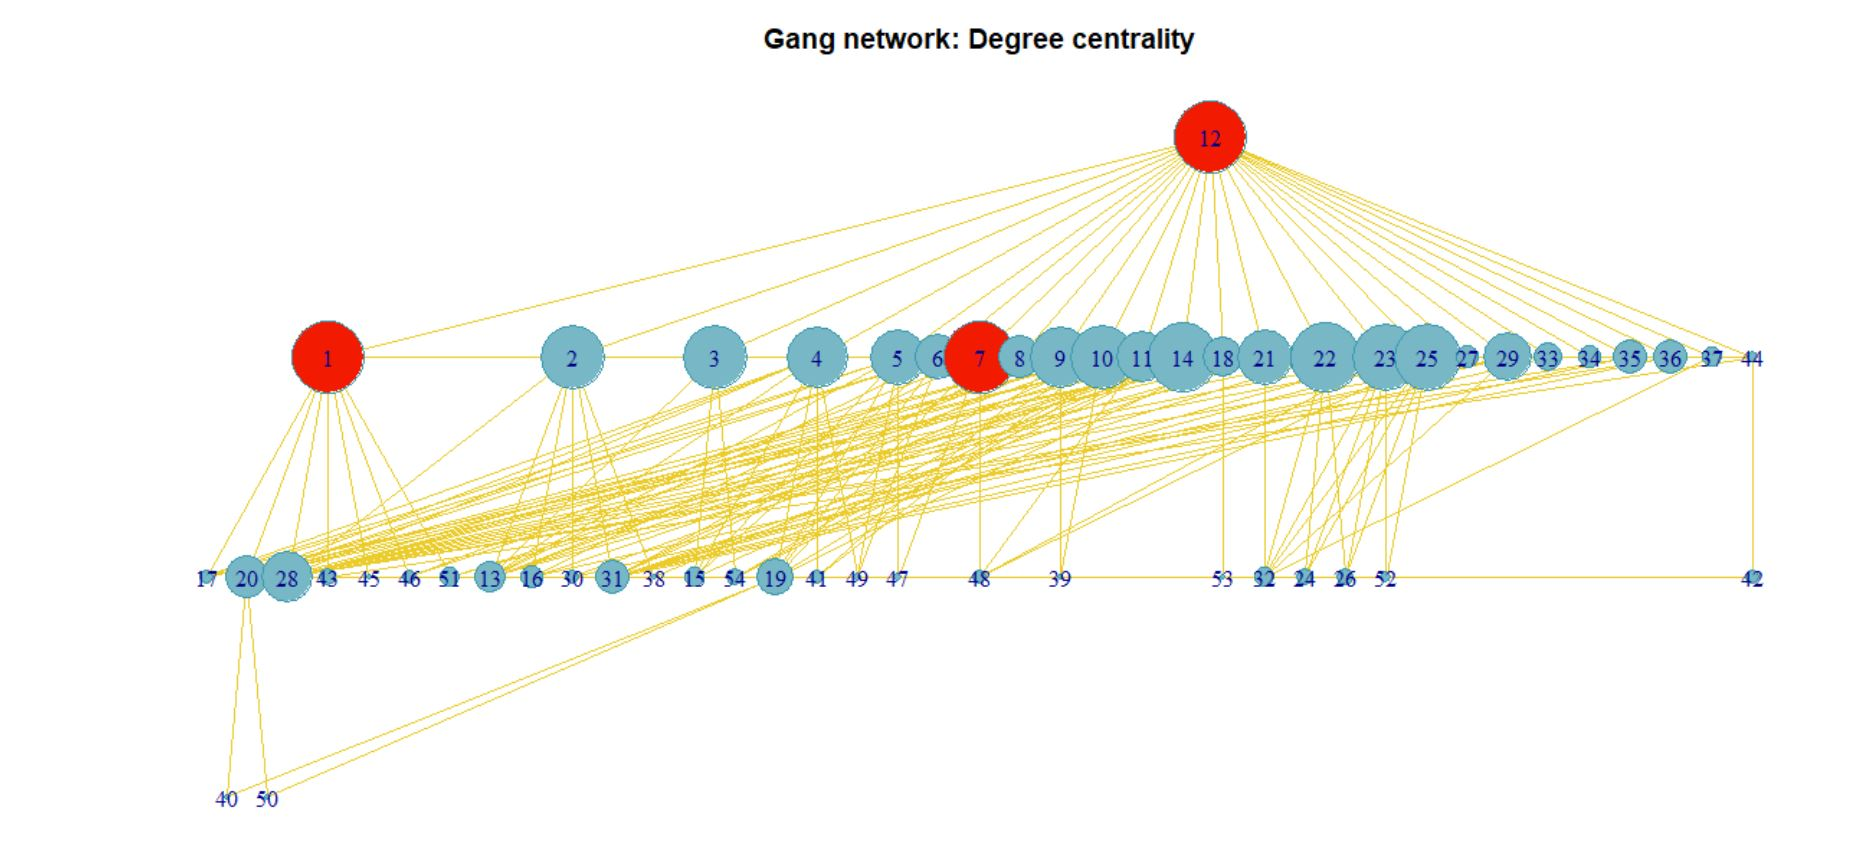
\includegraphics[scale =0.5]{degree}
	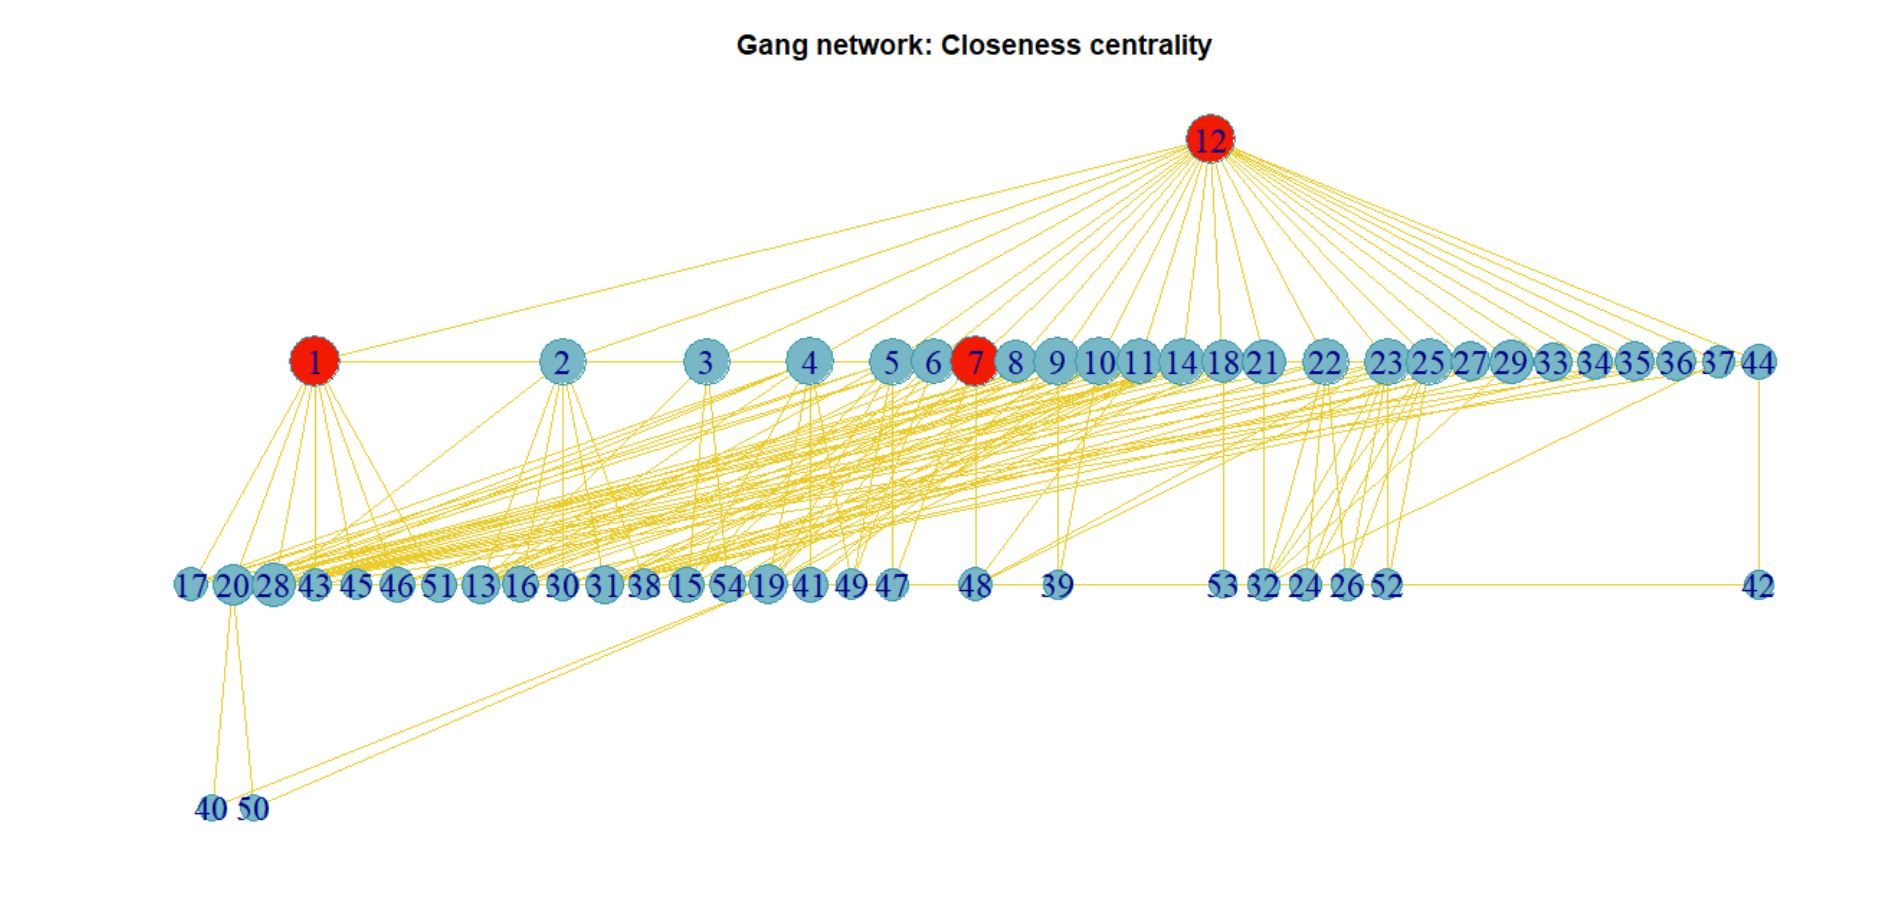
\includegraphics[scale =0.5]{closeness}

	
\end{figure}
\begin{figure}
	\centering
	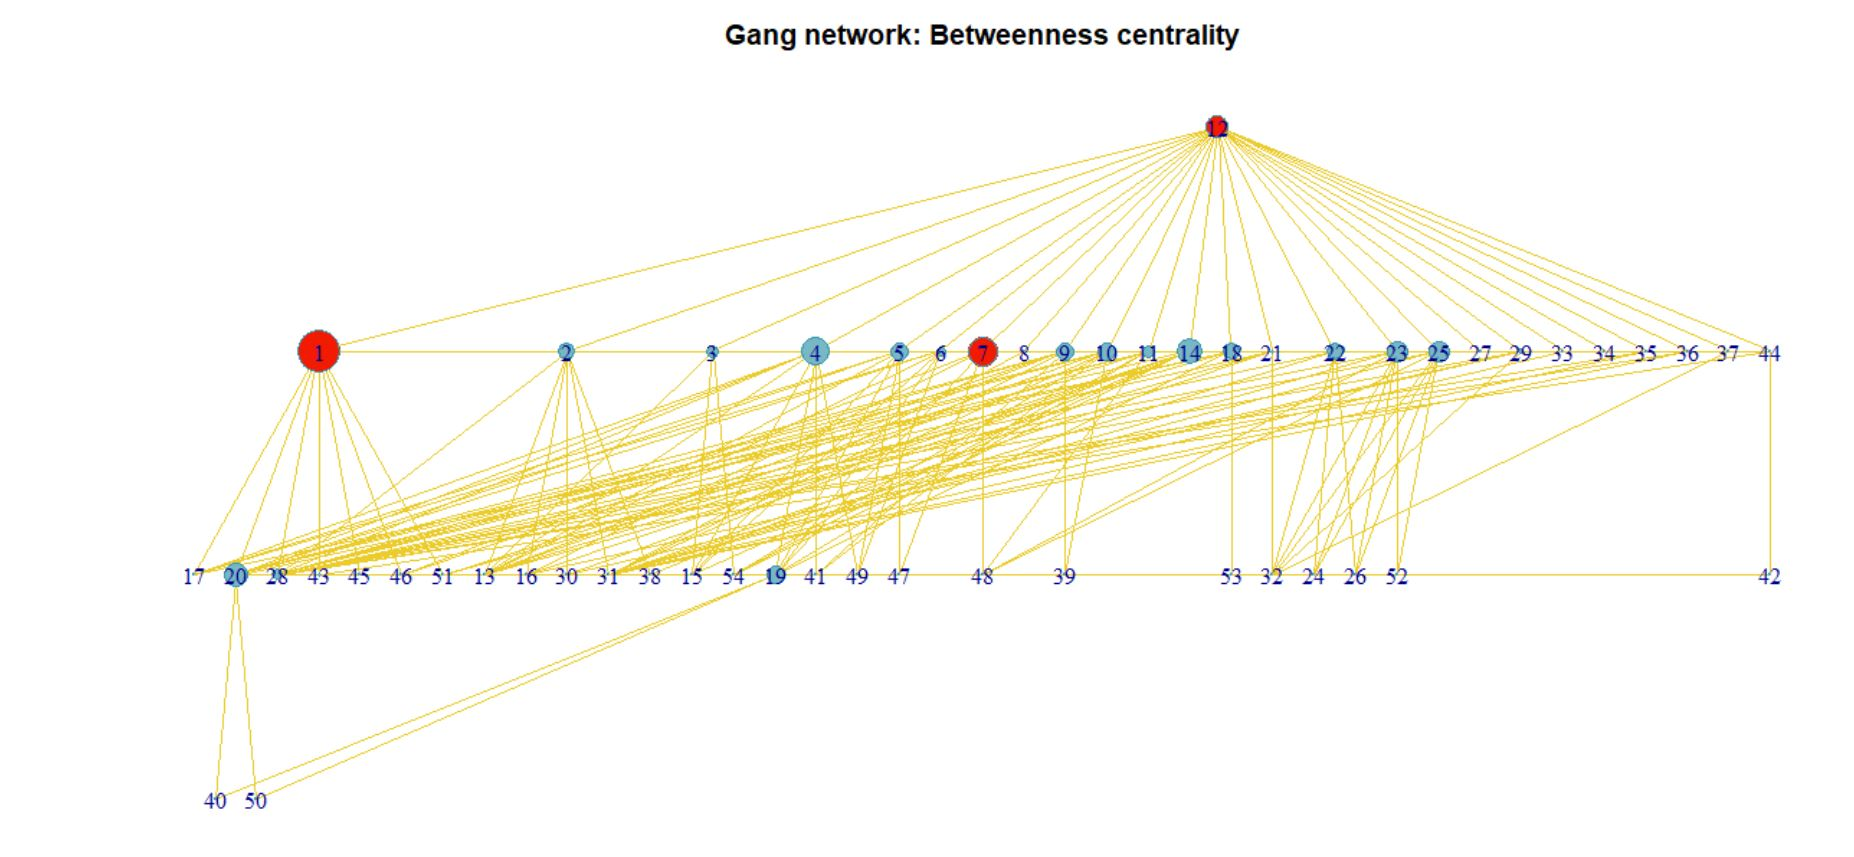
\includegraphics[scale =0.5]{betweeness}
	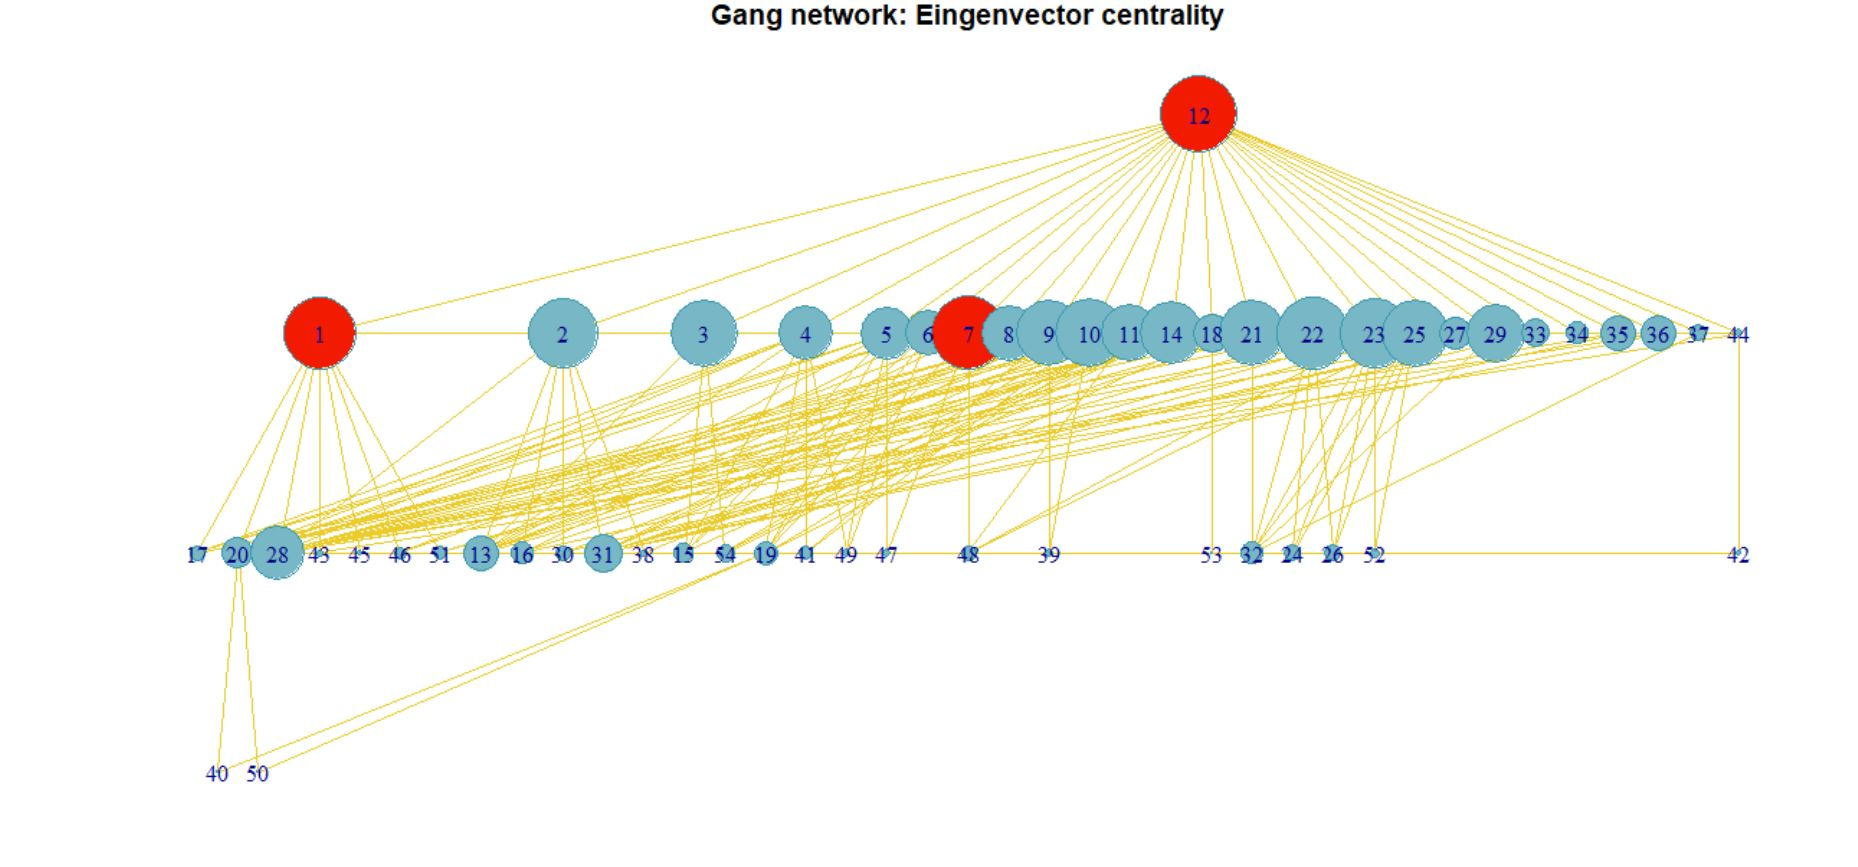
\includegraphics[scale =0.5]{ein}
\end{figure}

 Notiamo come nessun nodo del terzo o quarto livello risulti centrale, ovviamente questo \'e dovuto al tipo di organizzazione in esame. Mentre i nodi 1, 7 e 12 risultano sempre centrali, ovviamente il 12 lo \'e in quanto "capo" della gerarchia, mentre gli altri due nodi potrebbero essere i suoi diretti sottoposti, infatti essi risultano pi\'u centrali del 12 in termini di betweeness centrality, mentre hanno lo stesso peso nel senso di eigen vector centrality.
 \\
 Un modo per sintetizzare queste misure \'e quello di creare degli indici, i quali hanno un range che va da zero ad uno. Leggendo i risultati della tabella sottostante, si conferma ancora una volta la struttura del network, infatti  una Betweeness bassa indica la presenza di pochi capi, mentre la closeness rimarca la gerarchia delle associazioni a delinquere. \\
 \begin{center}
 \begin{tabular}{c|c}
 	\hline 
 	Tipo di centralit\'a & CI \\ 
 	\hline 
 	Degree &  0.2612482\\ 
 	\hline 
 	Closeness & 0.1555041 \\ 
 	\hline 
 	Betweeness & 0.003464251  \\ 
 	\hline 
 \end{tabular} 
 \end{center}
\chapter{Exponential Random Graph Model}
Successivamente \textbf{Y} indicher\'a la matrice di adiacenza e ${Y_{ij}}$ una suo valore.
\section{Modello Nullo: Random Graph Model}
Il Random Graph Model assume che ogni nodo ha la stessa probabilit\'a di essere osservato, indipendentemente dagli altri, ovvero:
$$ Y_{ij} \sim Bern(p) $$
Questo modello risulta un punto di partenza obbligatorio per la ricerca del nostro modello migliore, in quanto ci permette di chiarire il rischio di osservare un arco.
\\
Il modello usa un metodo di stima MLE, il termine dell'arco \'e il log-odds osservato (sotto l'assunzione di indipendenza), il segno negativo indica che la probabilit\'a di osservare un arco \'e inferiore a 0.5. 
\\
\begin{align*}
L(p) &= \prod_{i=1}^n p^{y_i}(1-p)^{(1-y_i)}\\
\ell(p) &= \log{p}\sum_{i=1}^n y_i + \log{(1-p)}\sum_{i=1}^n (1-y_i)\\
\dfrac{\partial\ell(p)}{\partial p} &= \dfrac{\sum_{i=1}^n y_i}{p} - \dfrac{\sum_{i=1}^n (1-y_i)}{1-p} \overset{\text{set}}{=}0\\
\sum_{i=1}^n y_i - p\sum_{i=1}^n y_i &= p\sum_{i=1}^n (1-y_i)\\
p& = \dfrac{1}{n}\sum_{i=1}^n y_i\\
\dfrac{\partial^2 \ell(p)}{\partial p^2} &= \dfrac{-\sum_{i=1}^n y_i}{p^2} - \dfrac{\sum_{i=1}^n (1-y_i)}{(1-p)^2}\\
&=-1.2649\\
(s.e. = 0.0638) 
\end{align*}
Il relativo odds \'e pari a 1.28, il coefficiente, risulta significativo, indi per cui la differenza tra la probabilit\'a di osservare o meno un arco \'e significativa.
\section{Modelli intermedi}
\subsection{Modello senza attributi}
Nel nostro framework l'interazione con pi\'u nodi, o specifici nodi, \'e centrale, in quanto definiscono il ruolo dell'unit\'a e la sua posizione gerarchica, inoltre anche gli attributi giocano un ruolo importante. La scelta naturale del modello ricade su un modello Markoviano, in quanto  assume la dipendenza delle diadi, ovvero:
$$Y_{ij} \not\!\perp\!\!\!\perp Y_{kl} se \{i, j\} \cap \{k, l\} \neq \emptyset $$
Il modello di Markov viene rappresentato attraverso il grafico delle dipendenze, in particolare il legame tra $Pr(\textbf{Y}= \textbf{y})$ e questo tipo di grafo viene espresso nel teorema di Hammersley-Clifford. Il teorema afferma che la probabilit\'a del modello per \textbf{Y} \'e definita solo dalle cliques presenti nel suo grafo delle dipendenze.
\\
Il modello generale risulta essere:
$$
Pr(\textbf{Y} = \textbf{y}) = \kappa^{-1} \exp{\mu L(y) + \sigma_2 S_2 (y)+ \sigma_3 S_3(y)+ \dots + \sigma_{n-1} S_{n-1} + \tau T(y)}
$$
Dove $S_r$ e $T$ sono, rispettivamente, le r-star e i triangoli osservati.
\\
Ovviamente per facilitare la stima dei coefficienti del modello \'e necessario fare delle assunzioni di omogeneit\'a, ovvero affermare che gli effetti delle r-str e dei triangoli siano uguali per tutti i nodi.
\\
Come \'e noto il modello cos\'i definito ha problemi di identificabilit\'a, indi per cui \'e necessario snellire il carico degli stimatori, ovvero bisogna trovare una soluzione al fatto che il modello degeneri e non arrivi a una vera e propria stima, per via dei pochi dati a disposizione.
\\
Usando un approccio partial conditional, aggiriamo la degenery iusses e riusciamo finalmente ad avere il modello, inserendo come covariate  i k-tringoli alternati e i k-star alternati.
\\
Il modello finale scelto risulta essere quello contente solo i k-triangoli alternati. Di seguito \'e riportato l'output.
\begin{figure}[H]
	\centering
	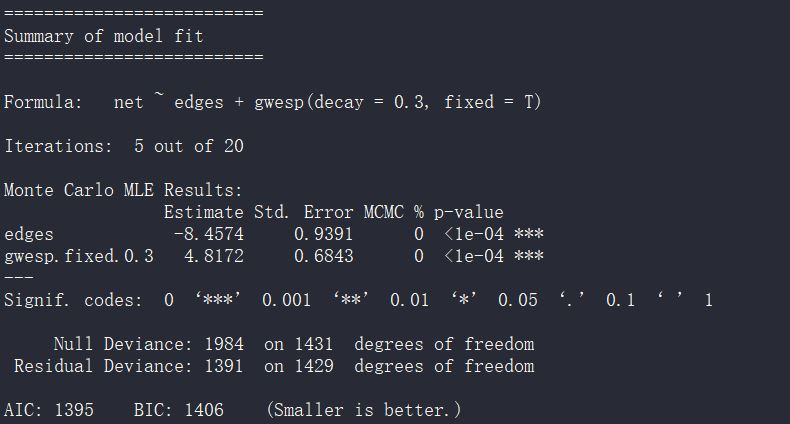
\includegraphics[scale=0.75]{mod1}
\end{figure}
Il valore e il segno dei parametri conferma quanto detto in precedenza, ovvero vi \'e una bassa probabilit\'a di osservare archi, ma una tendenza positiva a costruire triangoli, in questo caso alternati, tutti tratti distintivi di network con cluster o comunque con strutture piramidali.
\\
Insieme al modello cambia anche il metodo di stima, in questo caso viene usato l'MCMCLE, ovvero il Markov chain Monte Carlo Maximum Likelihood estimation. L'algoritmo stima un vettore di parametri attraverso un metodo di ottimizzazione per la likelihood, successivamente vengono pescate diverse matrice di adiacenza usando lo stesso vettore e infine si aggiorna il parametro, i due passi vengono iterati fino alla convergenza.
\\
Risulta fondamentale la scelta del punto di inizio, e obbligatorio il controllo della convergenza della catena.
\begin{figure}[H]
	\centering
	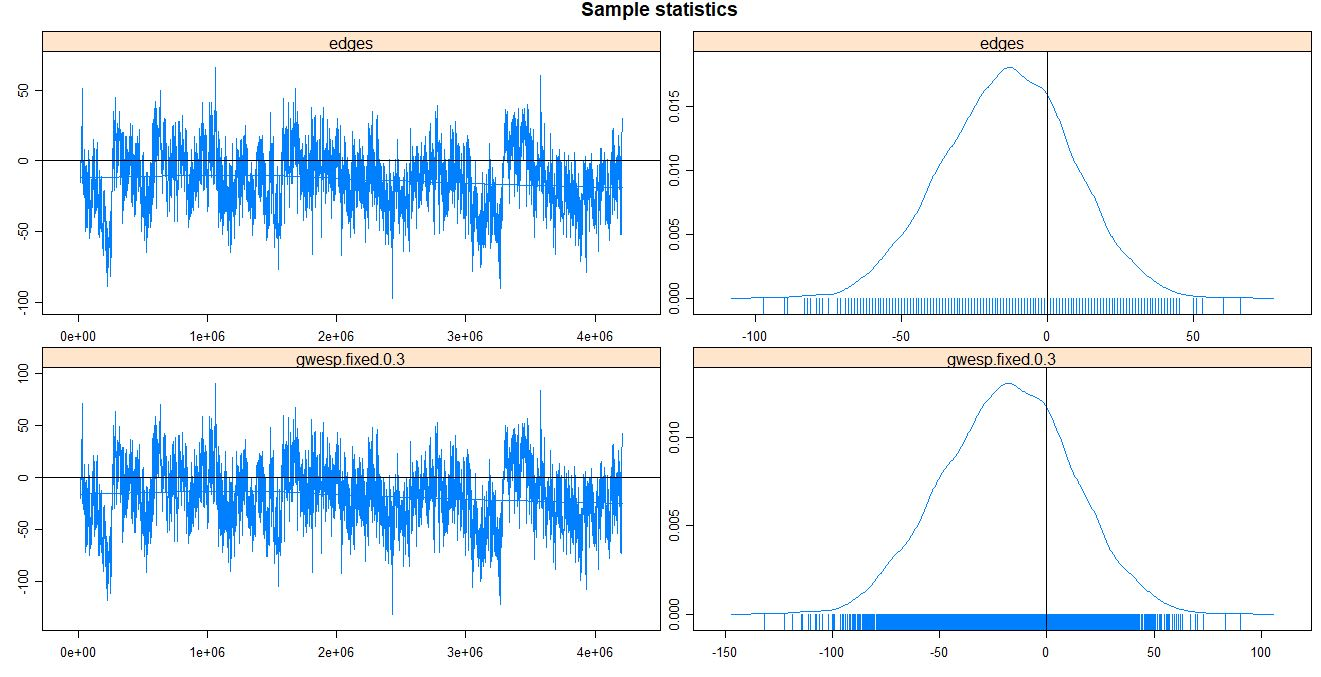
\includegraphics[scale=0.5]{mcmc1}
	\caption{La catena sembra converga in modo corretto.}
\end{figure}


\subsection{Modello con gli attributi}
Definiamo ora l'effetto di omifilia, ovvero quello che misura quanto forte un nodo con un certo attributo x tende a essere connesso con altri nodi aventi lo stesso attributo. In questa analisi ha senso considerare solo questo effetto, che pu\'o essere visto come tendenza di connessioni all'interno di un cluster.
\\
Il modello migliore risulta essere quello contente il luogo di nascita, gli arresti, le condanne e le et\'a, queste tre crateristiche sono molto legate tra di loro, infatti il luogo di nascita media tutti gli effetti.
\\
\begin{figure}[H]
	\centering
	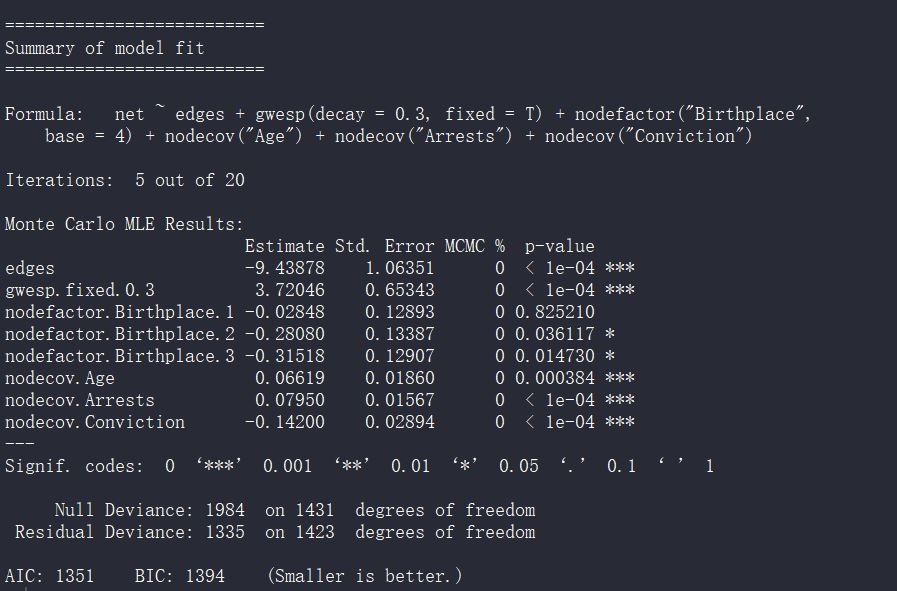
\includegraphics[scale=0.75]{mod2}
\end{figure}
Tutti i parametri degli attributi dicotomici positivi hanno un effetto di omofilia positivo, quelli negativi viceversa. Per Age invece, il segno positivo indica una alta attivit\'a dei nodi con un'et\'a alta, ci\'o \'e spiegato dal fatto che chi ha pi\'u anni \'e pi\'u in alto nella gerarchia.
\\
\begin{figure}[H]
	\centering
	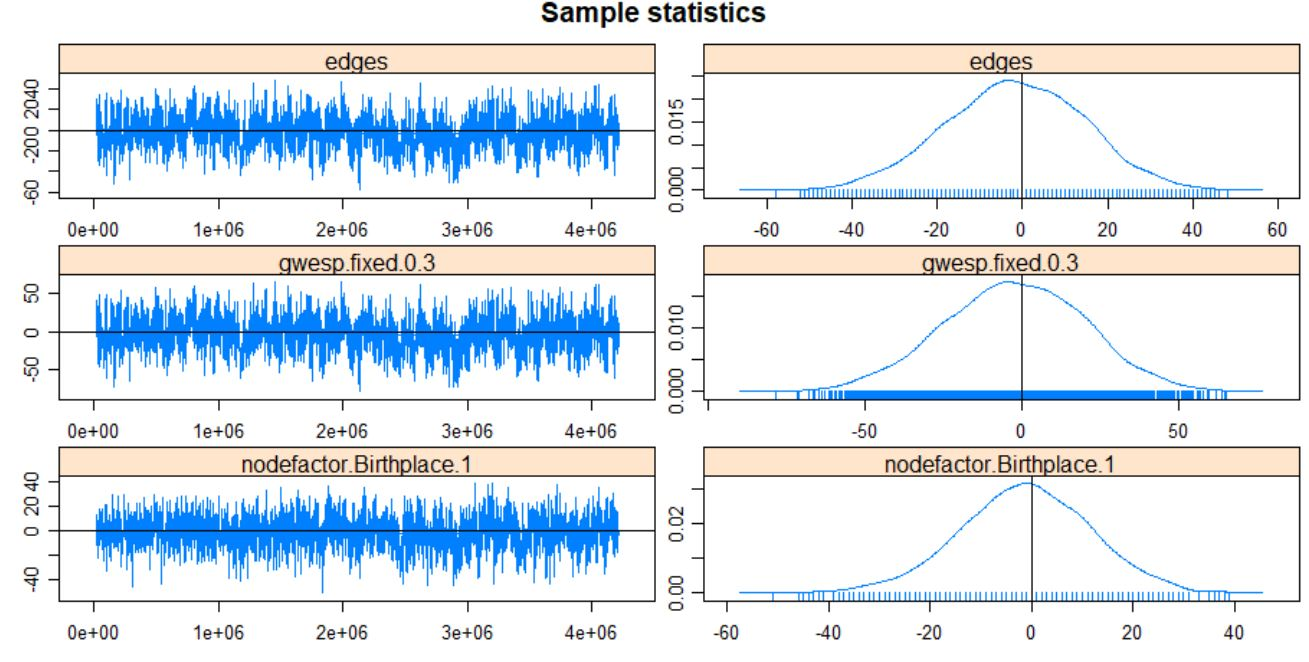
\includegraphics[scale=0.45]{mcmc2}
	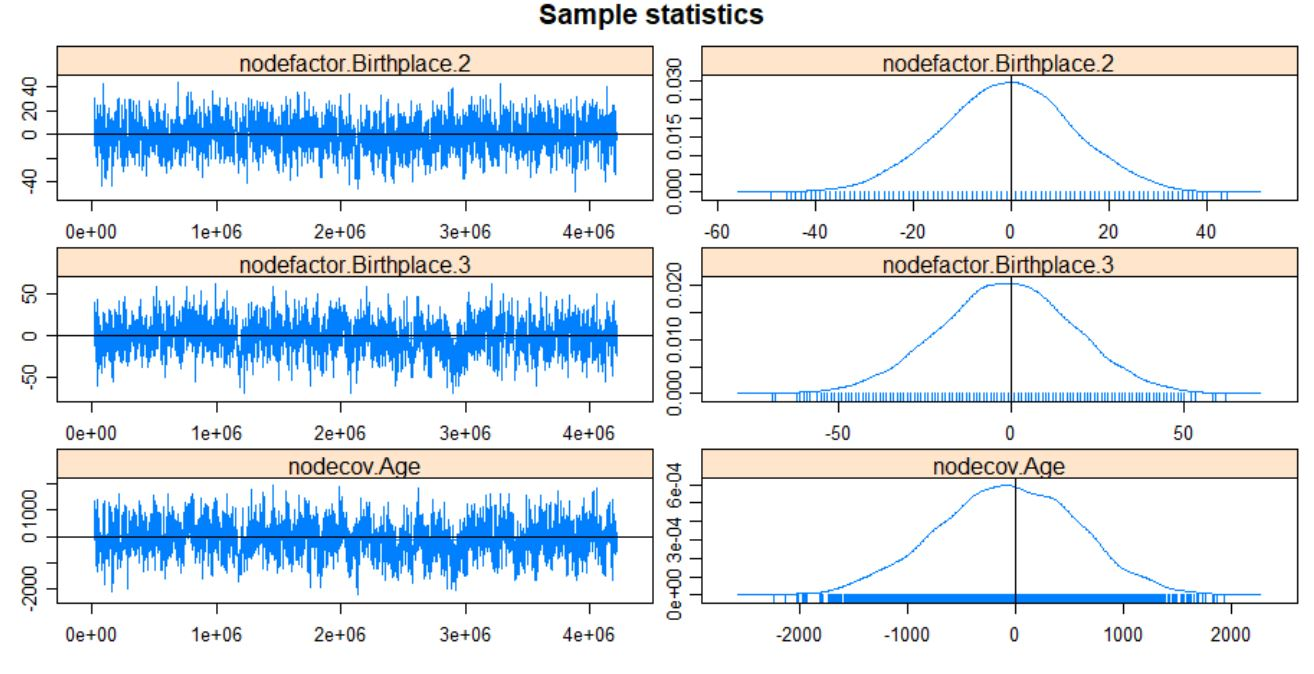
\includegraphics[scale=0.45]{mcmc3}
	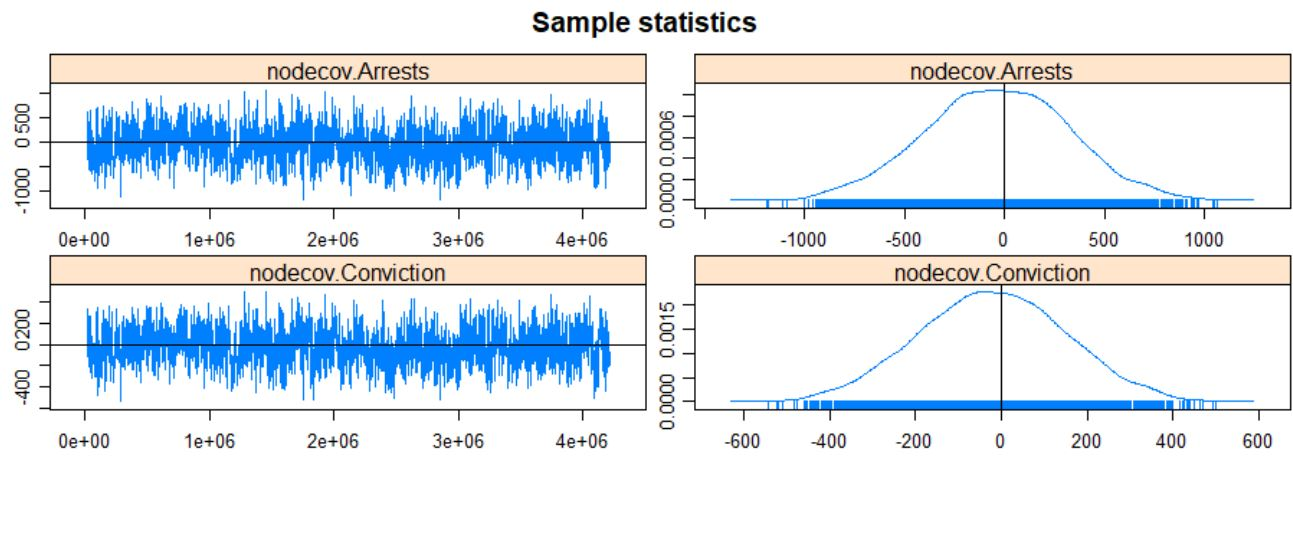
\includegraphics[scale=0.45]{mcmc4}
	\caption{il modello sembra avere una buona convergenza}
\end{figure}

\begin{figure}
	\centering
	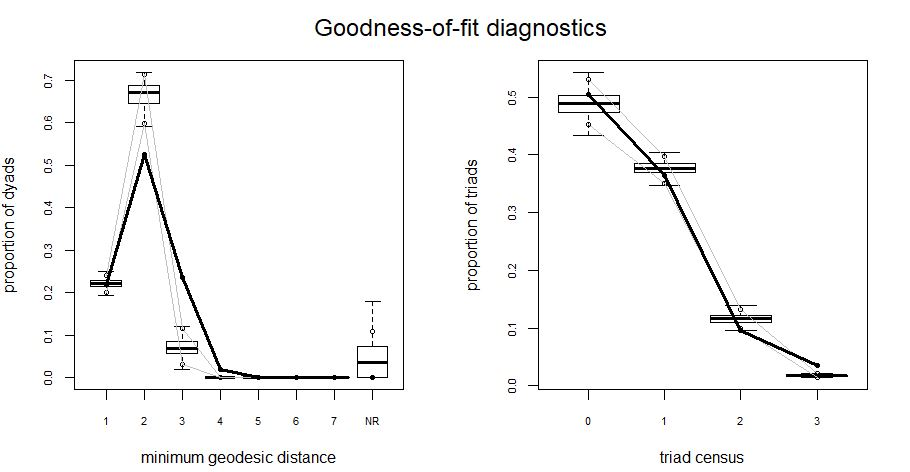
\includegraphics{gof}
	\caption{Il grafico riassume la bont\'a di adattemto, la quale risulta non essere buona per le distanze geodesic, mentre \'e molto buona per le triadi.}
\end{figure}
\chapter{Modello a blocchi latenti}
Con il modello a blocchi latente possiamo migliorare la comprensione del ruolo giocato dal luogo di nascita. 
\\
Anzitutto ricordiamo che questo modello ha la probabilit'a di osservare un legame che dipende solo dal proprio gruppo di appartenenza, in altre parole: i nodi sono indipendenti dato il gruppo di appartenenza.
\\
Stimato come 4 il numero di cluster pi\'u adatti, osserviamo le probabilit\'a a priori di appartenenre a ciascun gruppo.
\\
\\
\begin{tabular}{c|c|c|c|c}
	\hline 
	Probabilit\'a apriori di ciascun gruppo &       0.1352106& 0.2608365& 0.3953422& 0.2086108 \\ 
	\hline 
\end{tabular} 
\\
\\
Mentre le probabilit\'a a posteriori di osservare un arco tra e nei vari gruppi sono riportate nella tabella seguente.
\\
\begin{center}
\begin{tabular}{c|c|c|c|c}
		
		&  G1&  G2 & G3 &  G4\\ 
		\hline 
		G1&  0.572 &  0.478& 0.047 &  0.402
		\\ 
		\hline 
		G2&  0.478  &0.377   & 0.101  & 0.000 \\ 
		\hline 
		G3& 0.047  & 0.101 & 0.071  &0.000   \\ 
		\hline 
		G4& 0.402 &0.000&  0.000    & 0.224  \\ 
		\hline
		\hline
		\textbf{Numerosit\'a}&9 & 13 & 21& 11\\ 
	\end{tabular} 
\end{center}
Si noti che alcune probabilit\'a sono pari a zero, questo perch\'e avendo solo 54 osservazioni, non \'e possibile effettuare una perfetta analisi.
\\
Di seguito sono riportate le rappresentazioni grafiche dell'output della funzione \emph{mixer()}, insieme al boxplot che spiega la relazione tra i gruppi e il luogo di nascita.
\\
Particolarmente interessante \'e il confronto visivo tra il grafo colorato sotto le indicazioni del modello a blocchi latenti e quello riguardo l'attributo preso in esame. Essi risultano molto simili, ma data la bassa numerosit\'a dei gruppi, il modello non riesce a catturare tutti i punti.
\\
\begin{figure}[H]
	\centering
	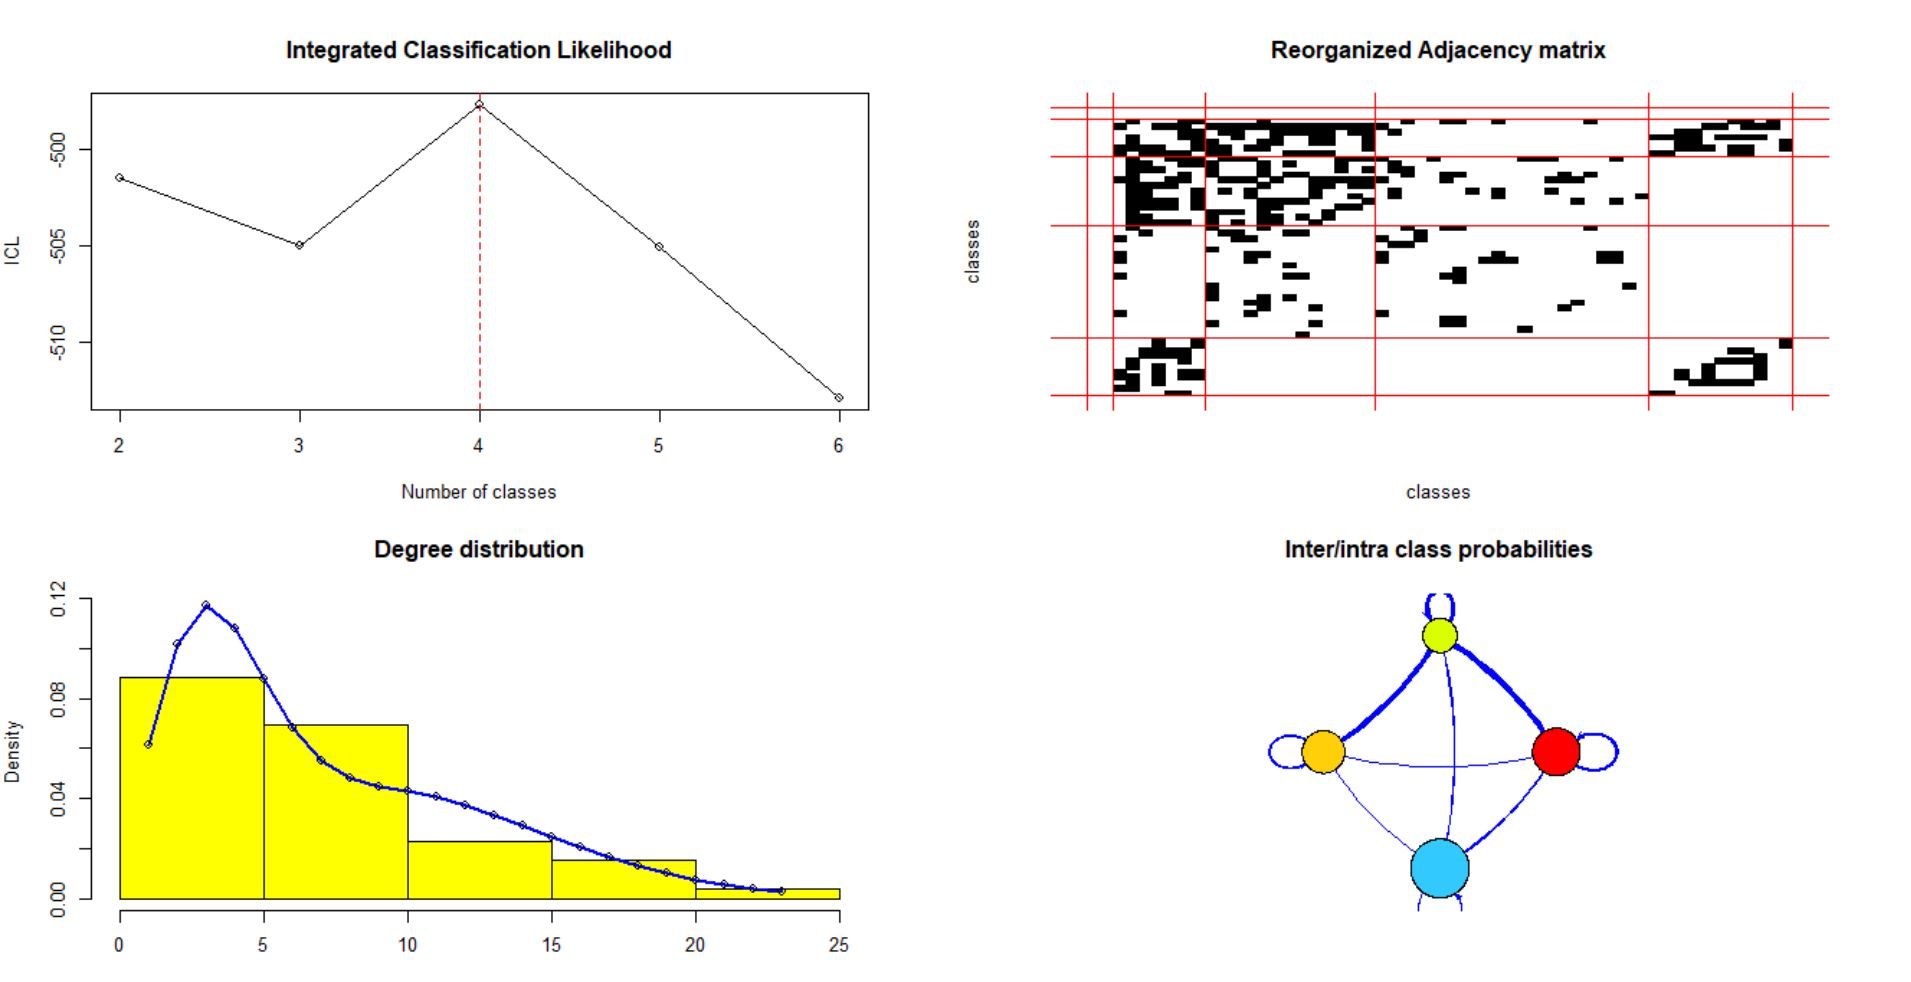
\includegraphics[scale=0.5]{Rplot}
	\caption{Summary grafico della funzione mixer.}
\end{figure}
\begin{figure}[H]
	\centering
	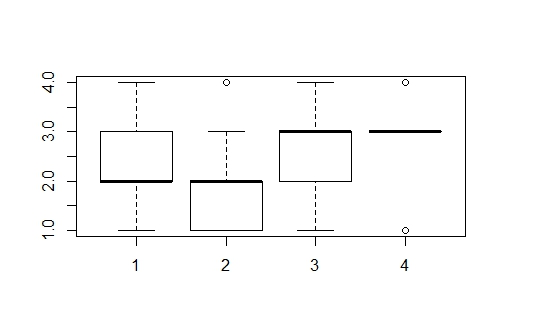
\includegraphics[scale=0.75]{boxplot}
	\caption{Box plot del luogo di nascita spiegato dai gruppi.}
\end{figure}
 
\begin{figure}[H]
	\centering
	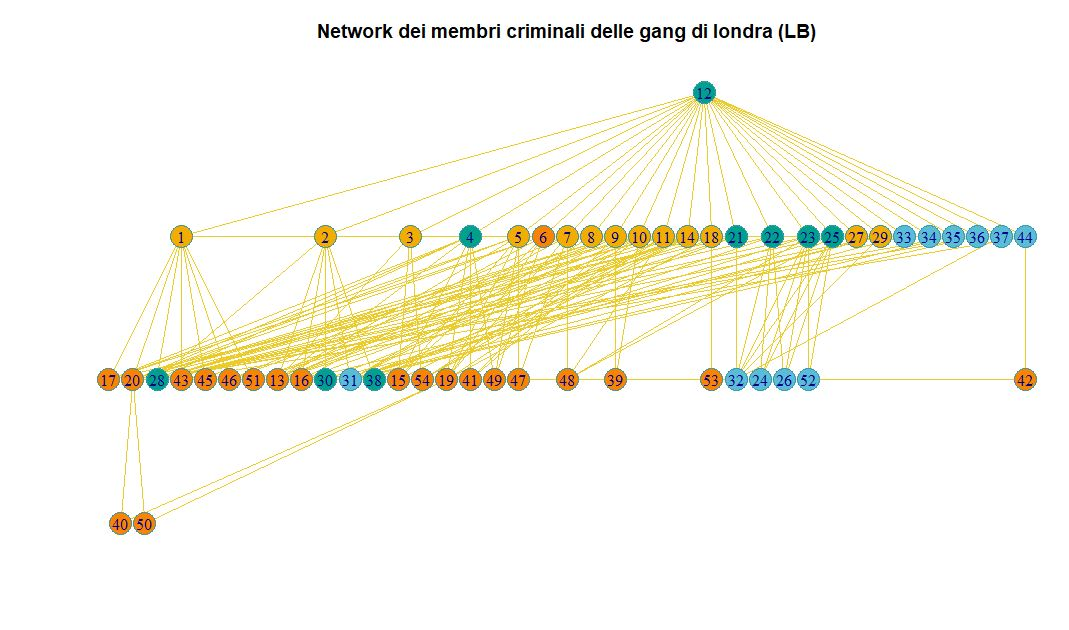
\includegraphics[scale=0.75]{last}
	\caption{In questa rappresentazione ogni colore del nodo rappresenta un gruppo diverso}
\end{figure}
\begin{figure}[H]
	\centering
	\includegraphics[scale =0.5]{BirthPlace}
	\caption{Sopra \'e riportato il grafo con i nodi colorari in base al luogo di nascita, il rosso indica i nati in Africa dell'ovest , il verde chi \'e dei Caraibi, il giallo \'e per i nati negli UK, l'arancione \'e per quelli dell'Africa dell'est}
	
	
\end{figure}
\chapter*{Appendice}
Di seguito sono riportati gli output dei modelli che hanno contribuito a spiegare al meglio il ruolo dell'attributo \emph{Birthplace}.
\begin{figure}[H]
	\centering
	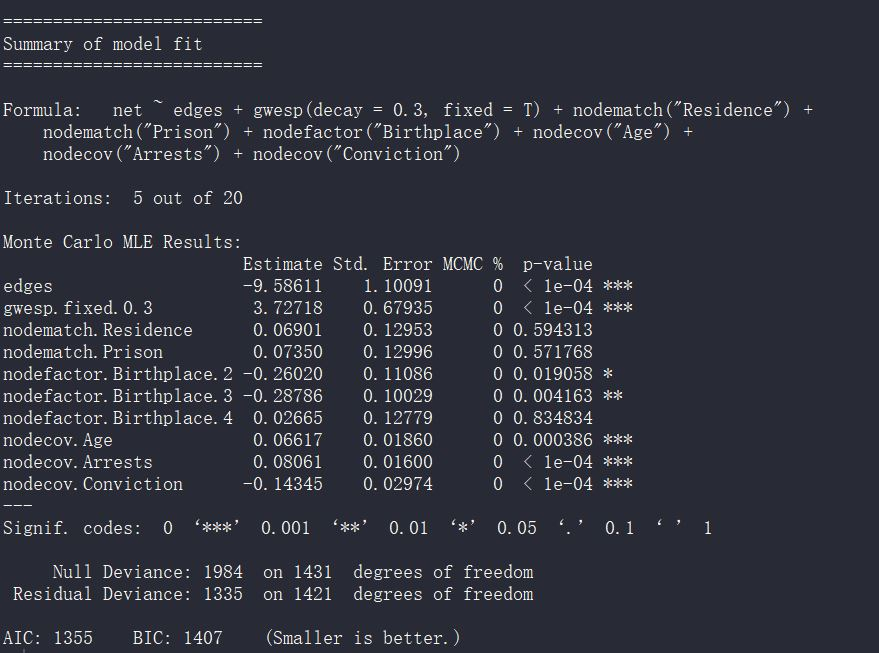
\includegraphics[scale =0.7]{modcov}
	\caption{Modello completo con tutti gli attributi }
		
\end{figure}
\begin{figure}[H]
	\centering
	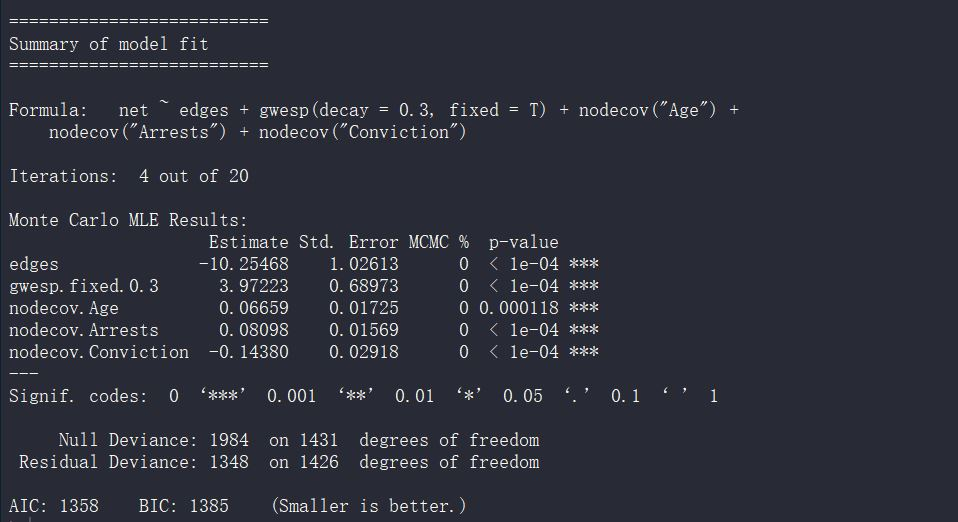
\includegraphics[scale =0.7]{modcov3}
	\caption{Modello completo senza l'attributo \emph{Birthplace} }
\end{figure}

\begin{figure}
	\centering
	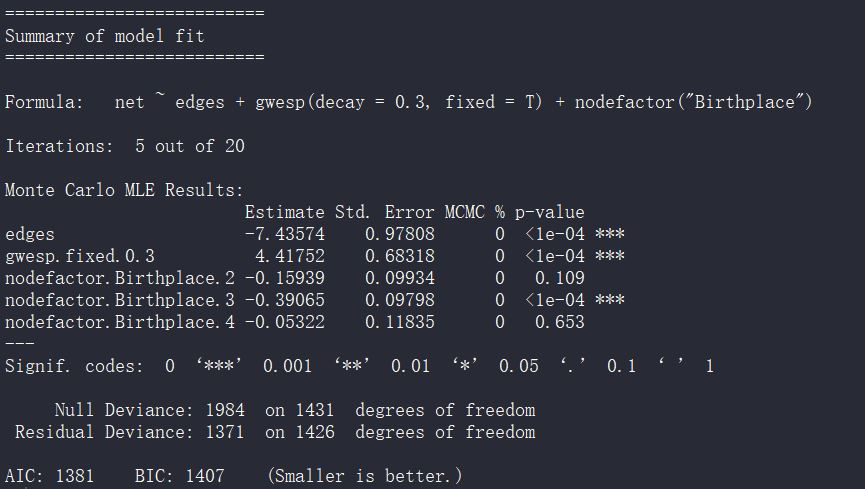
\includegraphics[scale =0.7]{modcov4}
	\caption{Modello con l'attributo \emph{Birthplace} }
\end{figure}

\begin{figure}
	\centering
	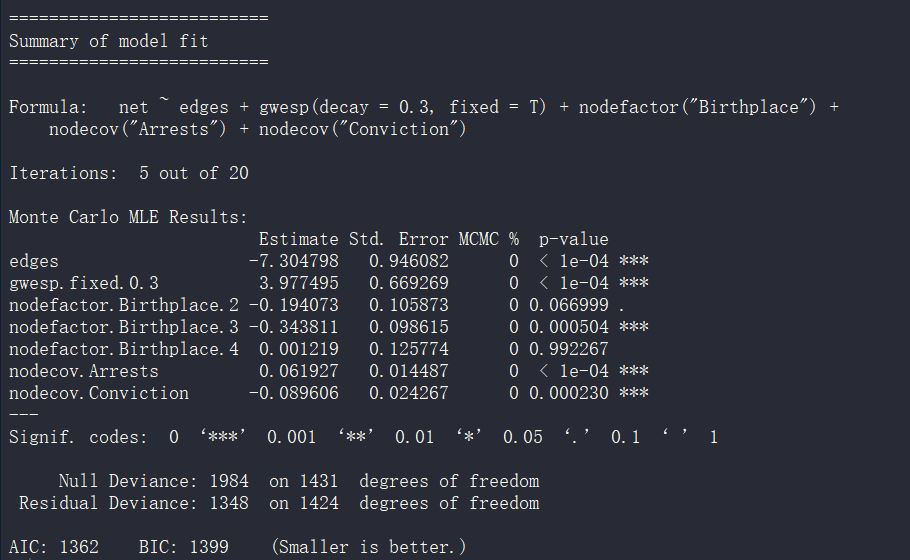
\includegraphics[scale =0.7]{mod5}
	\caption{Modello completo senza l'attributo \emph{Age} }
\end{figure}


\chapter*{Riferimenti}
Grund, T. and Densley, J. (2015) Ethnic Homophily and Triad Closure: Mapping Internal Gang Structure Using Exponential Random Graph Models. Journal of Contemporary Criminal Justice, Vol. 31, Issue 3, pp. 354-370

Grund, T. and Densley, J. (2012) Ethnic Heterogeneity in the Activity and Structure of a Black Street Gang. European Journal of Criminology, Vol. 9, Issue 3, pp. 388-406.
SOURCE: Available from Manchester.

\end{document}
